\section{Numerical Results and Comparisons}\label{sec:results}

\begin{figure}[!ht]
  \begin{centering}
  
\includegraphics[width=.8\columnwidth]{mesh}
  \caption{\label{fig:mesh} Initial coarse mesh (a),
  	half refined mesh (b) and refined mesh (c). The coarse mesh (a)
	and refined mesh (c) were used in the initial calculations, the latter one
	in case of \emph{p}-adaptivity (including HP\_ANISO\_P). The half-refined mesh was
	used later to optimize the \emph{hp}-adaptive refinement solutions.}
  \end{centering}
\end{figure}
Calculation for all the refinement modes were performed
in both single-mesh and multi-mesh configurations. 
The following numerical results were recorded for each 
refinement mode: converged relative error, cumulative CPU
time, and the problem size in terms of number
of degrees of freedoms (NDOFs) at each time step. 
Two types of initial meshes were used --- in case of only \emph{p}-adaptivity,
more refined mesh was used (Fig.~\ref{fig:mesh}~(c)) to ensure
the error convergence.
When the element size refinement
was also enabled (all \emph{h}/\emph{hp} refinement modes), very coarse initial mesh
was used (see Fig.~\ref{fig:mesh}~(a)) to let the adaptivity
algorithm find the most optimal mesh. That coarse initial mesh might not be
suitable for practical applications, as will be demonstrated in the
end of this section, however, it provides a good insight into the
adaptivity performance of Hermes.
In both cases, the initial mesh was loaded at each time step of the
calculation.

\begin{figure}[!ht]
  \begin{centering}
  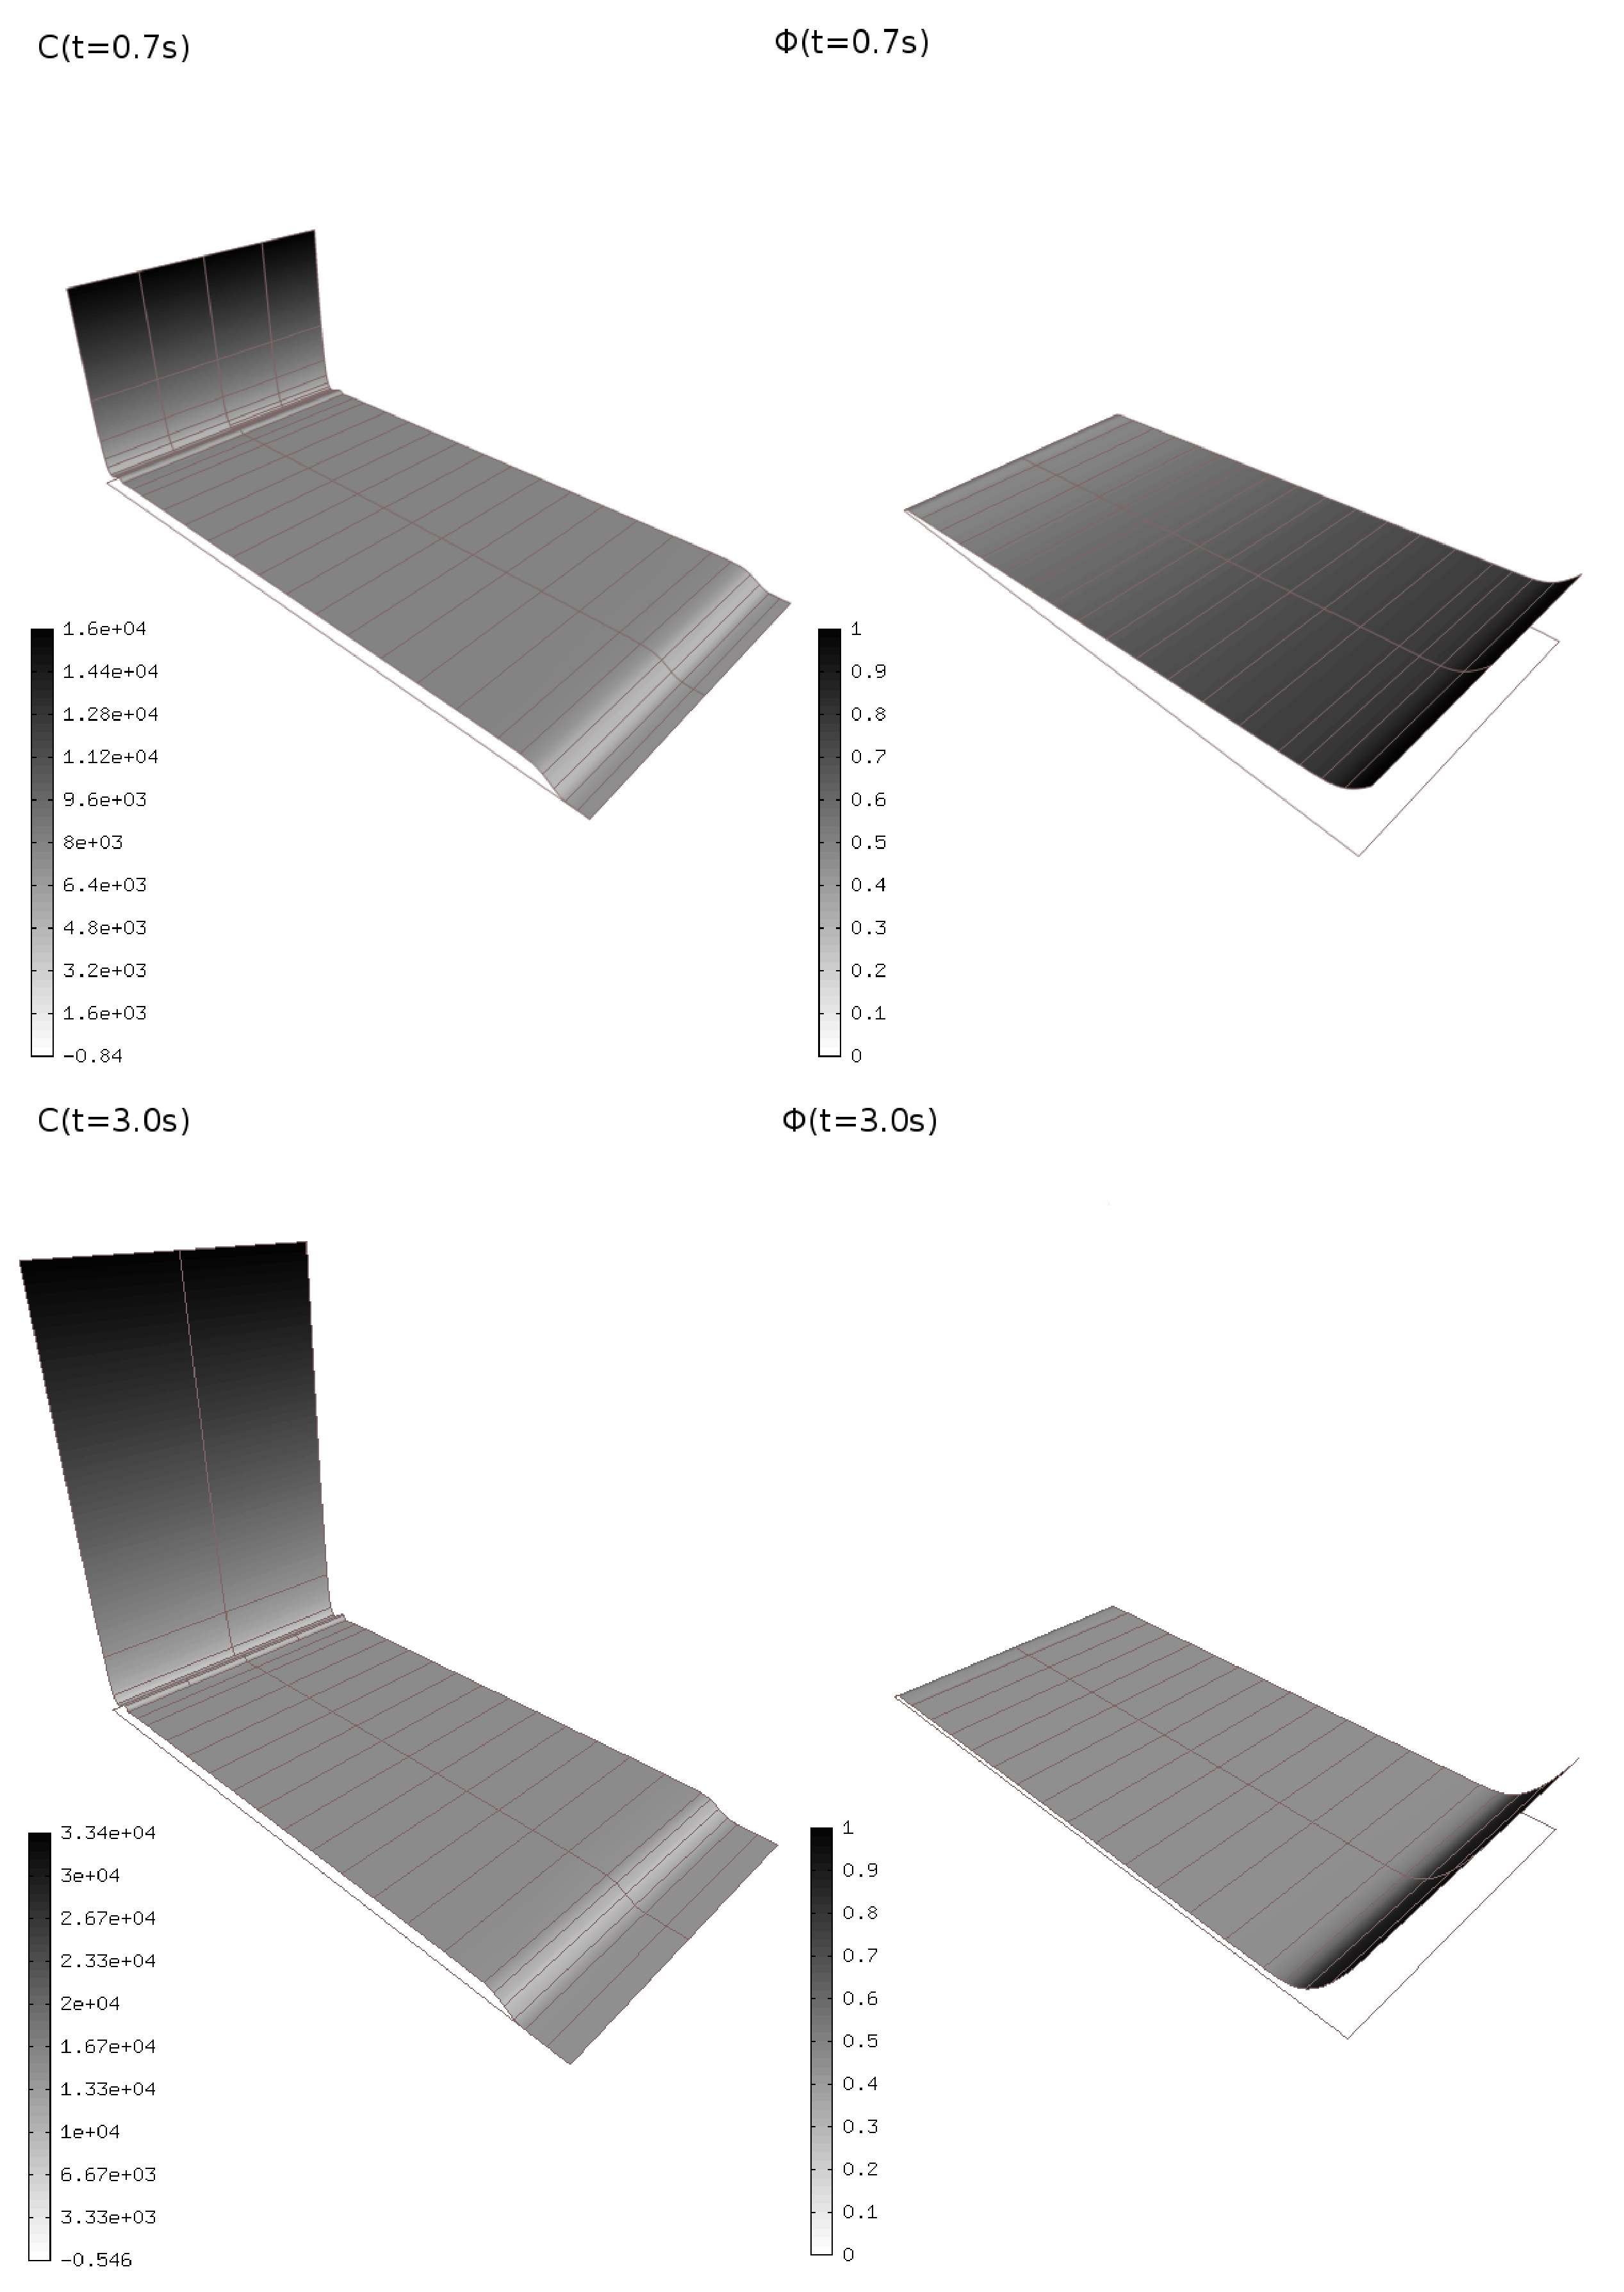
\includegraphics[width=.75\columnwidth]{cphi}
  \caption{\label{fig:cphi} Concentration $C$
  and voltage $\phi$ at two different time steps
  (HP\_ANISO refinement mode was used). This is a 2D solution shown
  in 3D, where the height indicates the values of $C$ and $\phi$.}
  \end{centering}
\end{figure}
Example of the solution at $t=0.7\ s$ and $t=3.0\ s$ 
calculated with HP\_ANISO refinement mode is shown
in Fig.~\ref{fig:cphi}. The time $t=0.7\ s$ was chosen because
by that time (with given constants in Table~\ref{Table:used-constants}),
some ionic migration has already taken place and
the concentration gradients near the boundaries $\partial\Omega_1$ and
$\partial\Omega_3$ have formed. The automatic mesh refinements
at different time steps are clearly visible in the figure --- especially
near $\partial\Omega_1$, where the $C_{\Omega_1}\approx 0$ and
the gradient $\nabla C$ is
shifting in time (this is also demonstrated in Fig.~\ref{fig:comsol-conc-volt}).

The following subsections provide a detailed comparison of
the different refinement modes and try to estimate the most suitable
one for the given problem.

\subsection{Optimal refinement modes}

\begin{figure}[!ht]
  \begin{centering}
  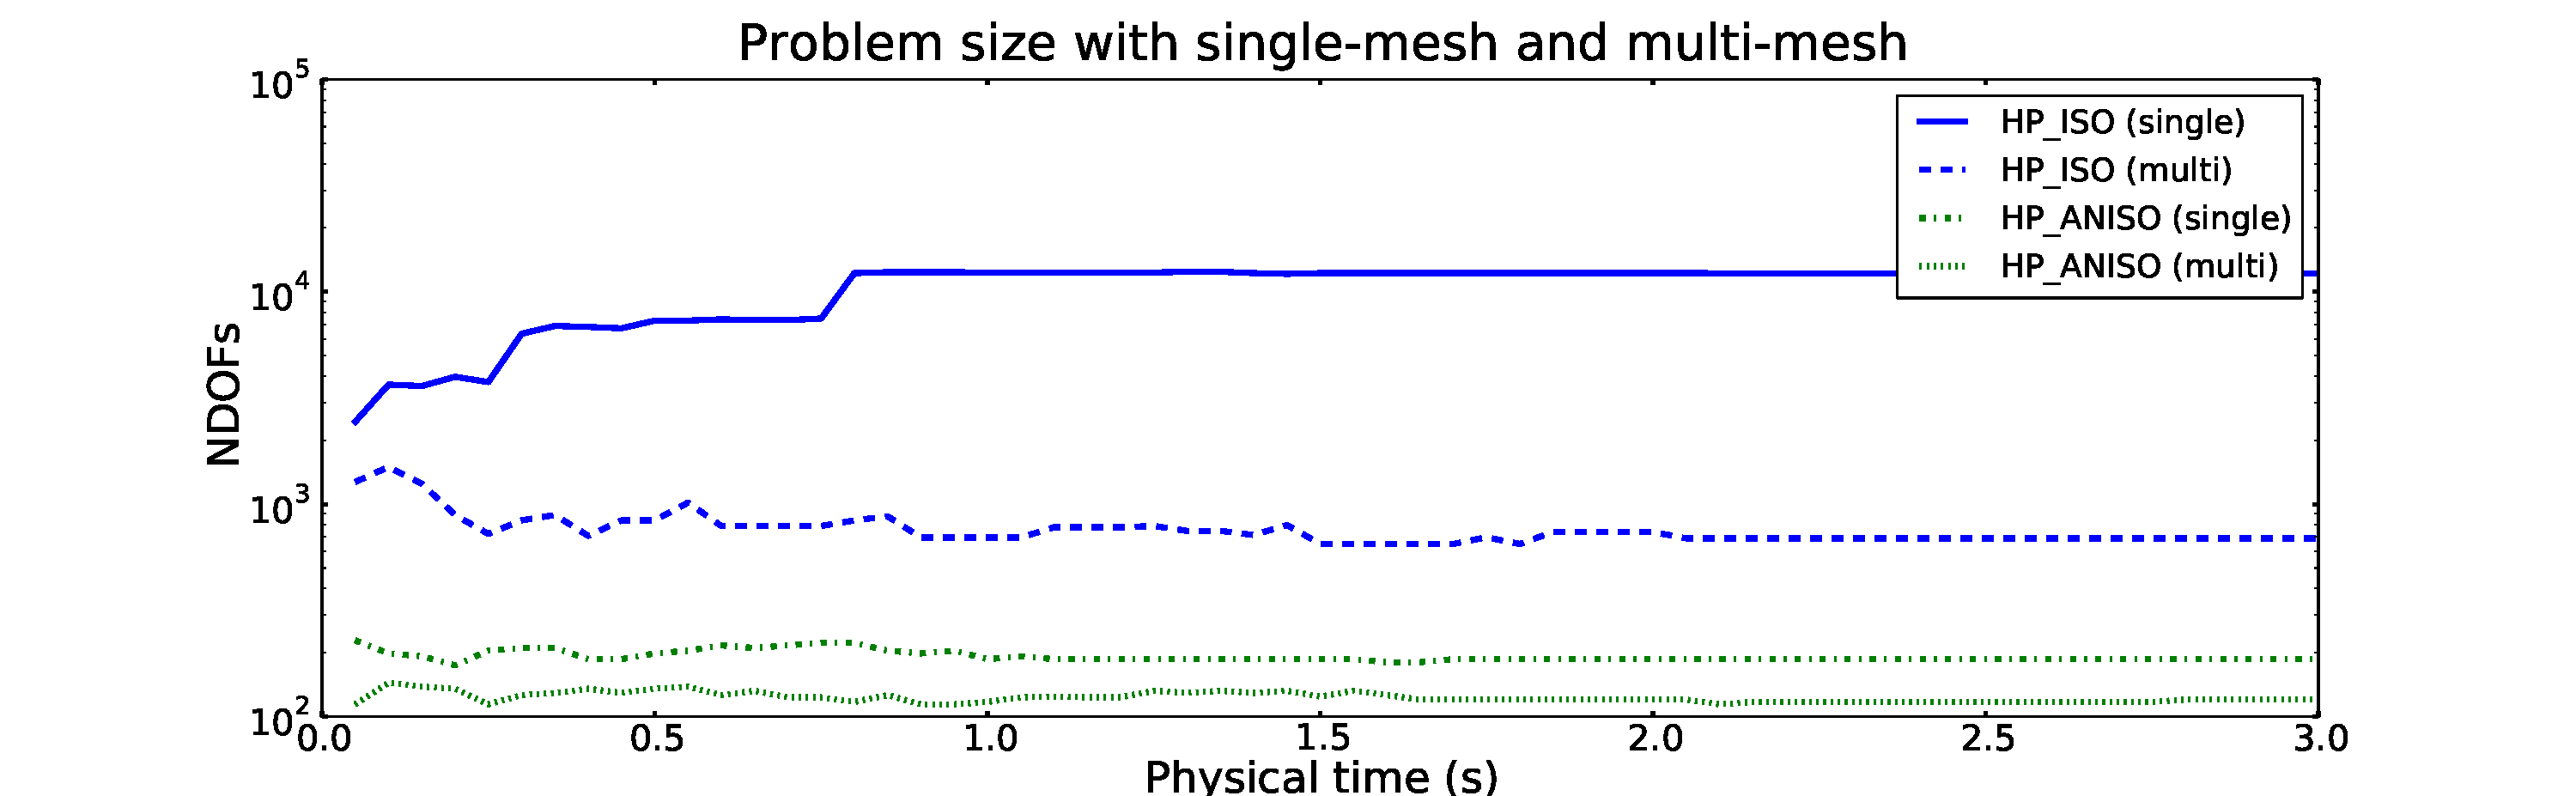
\includegraphics[width=\columnwidth]{singlemulti_dof}
  \caption{\label{fig:singlemultidof} NDOFs in case 
  of single-mesh and multi-mesh configurations with HP\_ISO
  and HP\_ANISO refinement modes. (Notice log Y scale)}
  \end{centering}
\end{figure}

\begin{figure}[!ht]
  \begin{centering}
  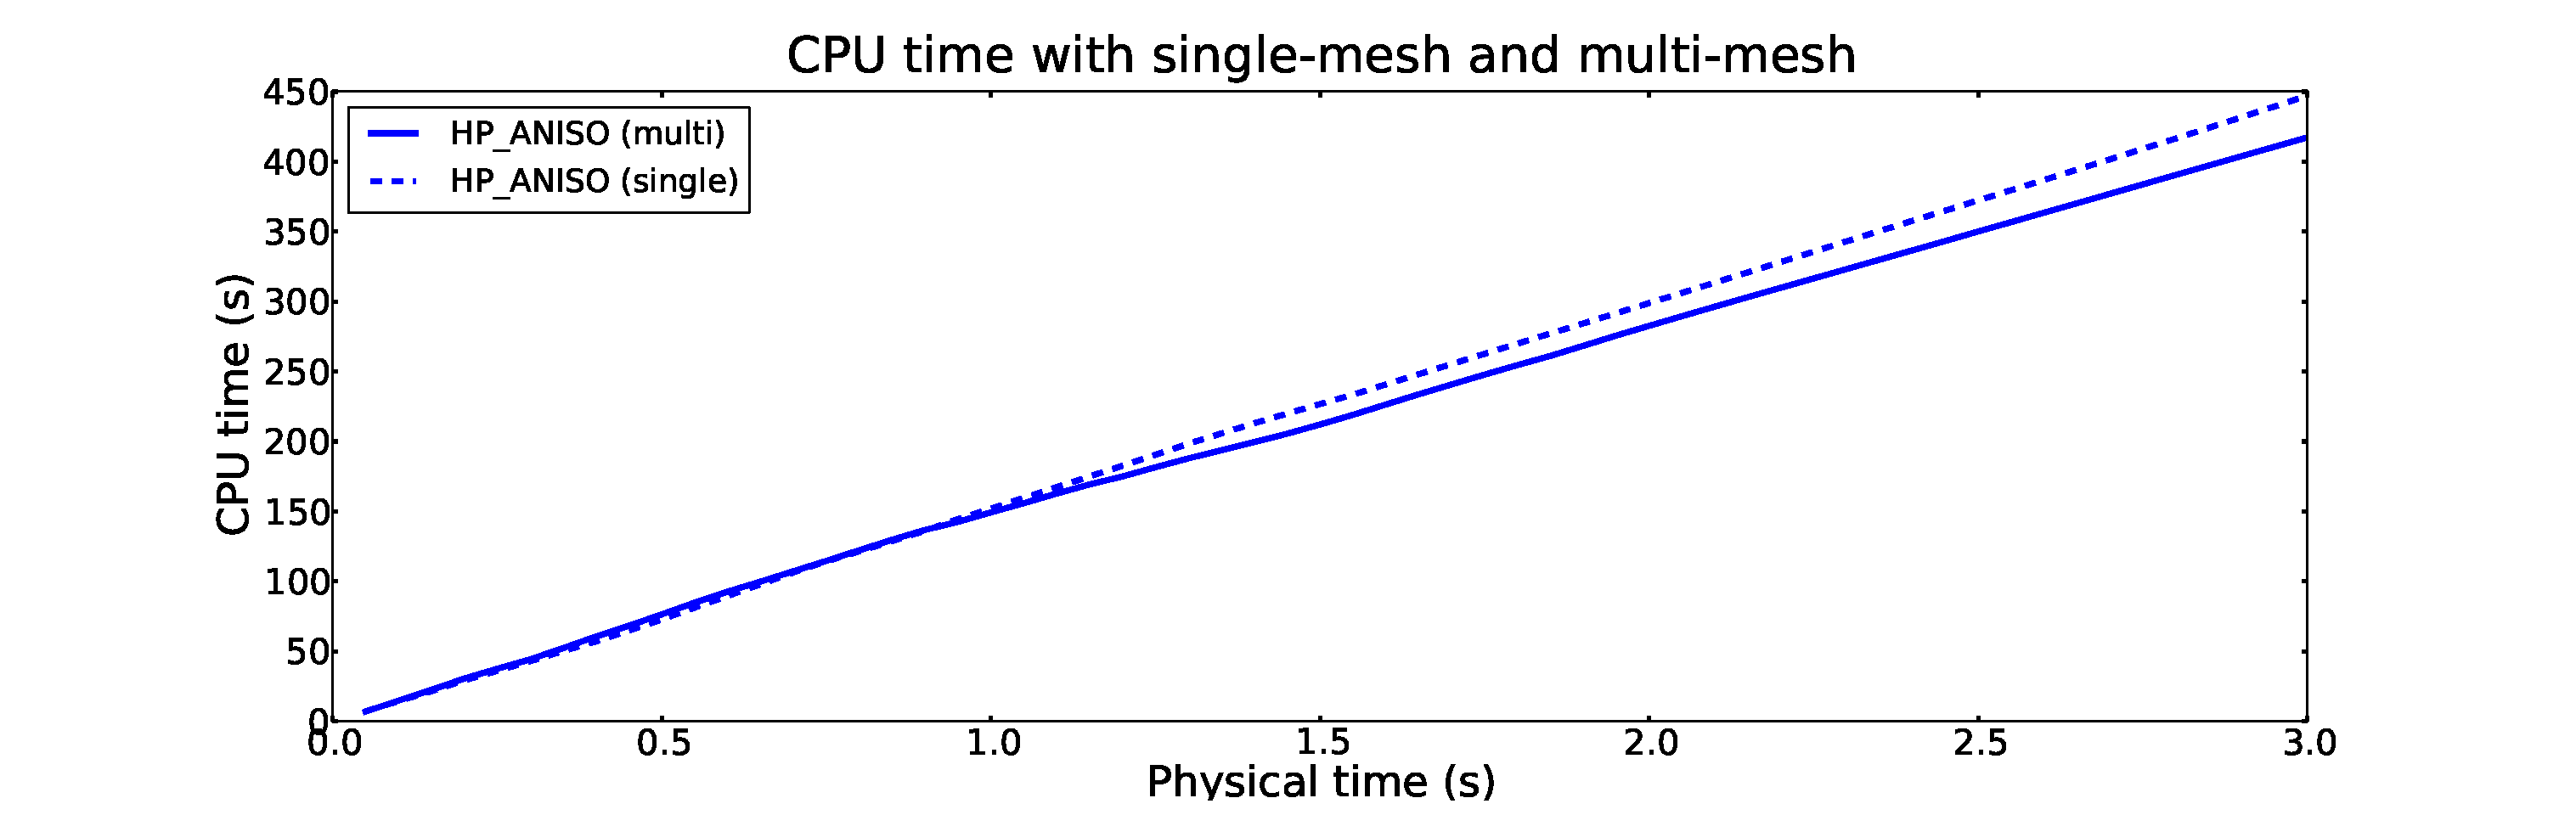
\includegraphics[width=\columnwidth]{singlemulti_cpu}
  \caption{\label{fig:singlemulticpu} Cumulative CPU times in case
  of single-mesh and multi-mesh configurations with HP\_ISO
  and HP\_ANISO refinement modes. (Notice log Y scale)}
  \end{centering}
\end{figure}

\begin{figure}[!ht]
  \begin{centering}
  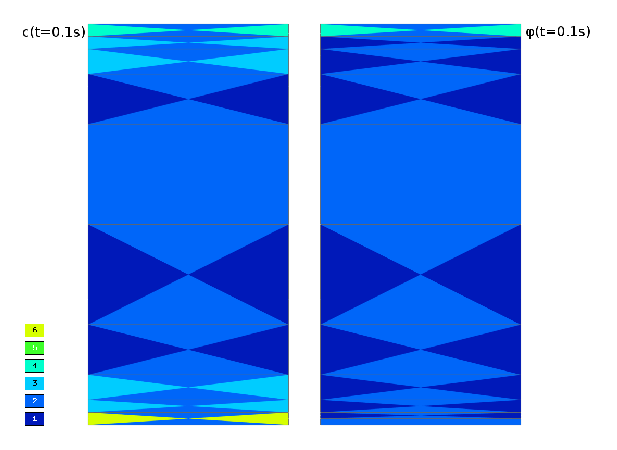
\includegraphics[width=.75\columnwidth]{poly}
  \caption{\label{fig:poly} Polynomial degree space
  for $C$ and $\phi$ at $t=0.7\ s$ The color indicates
  the maximum polynomial degree of the corresponding element.}
  \end{centering}
\end{figure}

Running the simulation with different refinement modes 
and meshes showed that the multi-mesh configuration generally results in
a smaller problem, faster calculation, and better or similar error convergence
compared to the single-mesh configuration.
This is well illustrated in Fig.~\ref{fig:singlemultidof} 
and Fig.~\ref{fig:singlemulticpu}.
The result can be understood when considering Fig.~\ref{fig:cphi} --- in the vicinity
of the boundaries $\partial \Omega_1$ and $\partial\Omega_3$ the concentration gradient
is greate than voltage gradient, namely $\nabla C >> \nabla \phi$. Therefore,
adapting the mesh for both variables is not reasonable in terms of
number of degrees of freedom. For instance,
the solution space with corresponding mesh in case of
HP\_ANISO at $t=0.7\ s$ is shown in Fig.~\ref{fig:cphi}. The corresponding polynomial
degree space for multi-mesh configuration is shown in Fig.~\ref{fig:poly}. 
Notice that the adaptivity algorithm
of Hermes has increased the maximum polynomial degree for the $C$-space to~7, however,
the maximum polynomial degree for the $\phi$-space is~2. Furthermore,
the mesh is significantly more refined for $C$.
For most of the cases using the multi-mesh results in similar or better CPU time.
It means that multi-mesh takes less computational resources. Only excpetion was HP\_ANISO\_H 
refinement mode for which the single mesh configuration resulted slightly faster
calculation time. 
Based on the results, only multi-mesh configurations will be considered
in the following comparisons.

\begin{figure}[!ht]
  \begin{centering}
  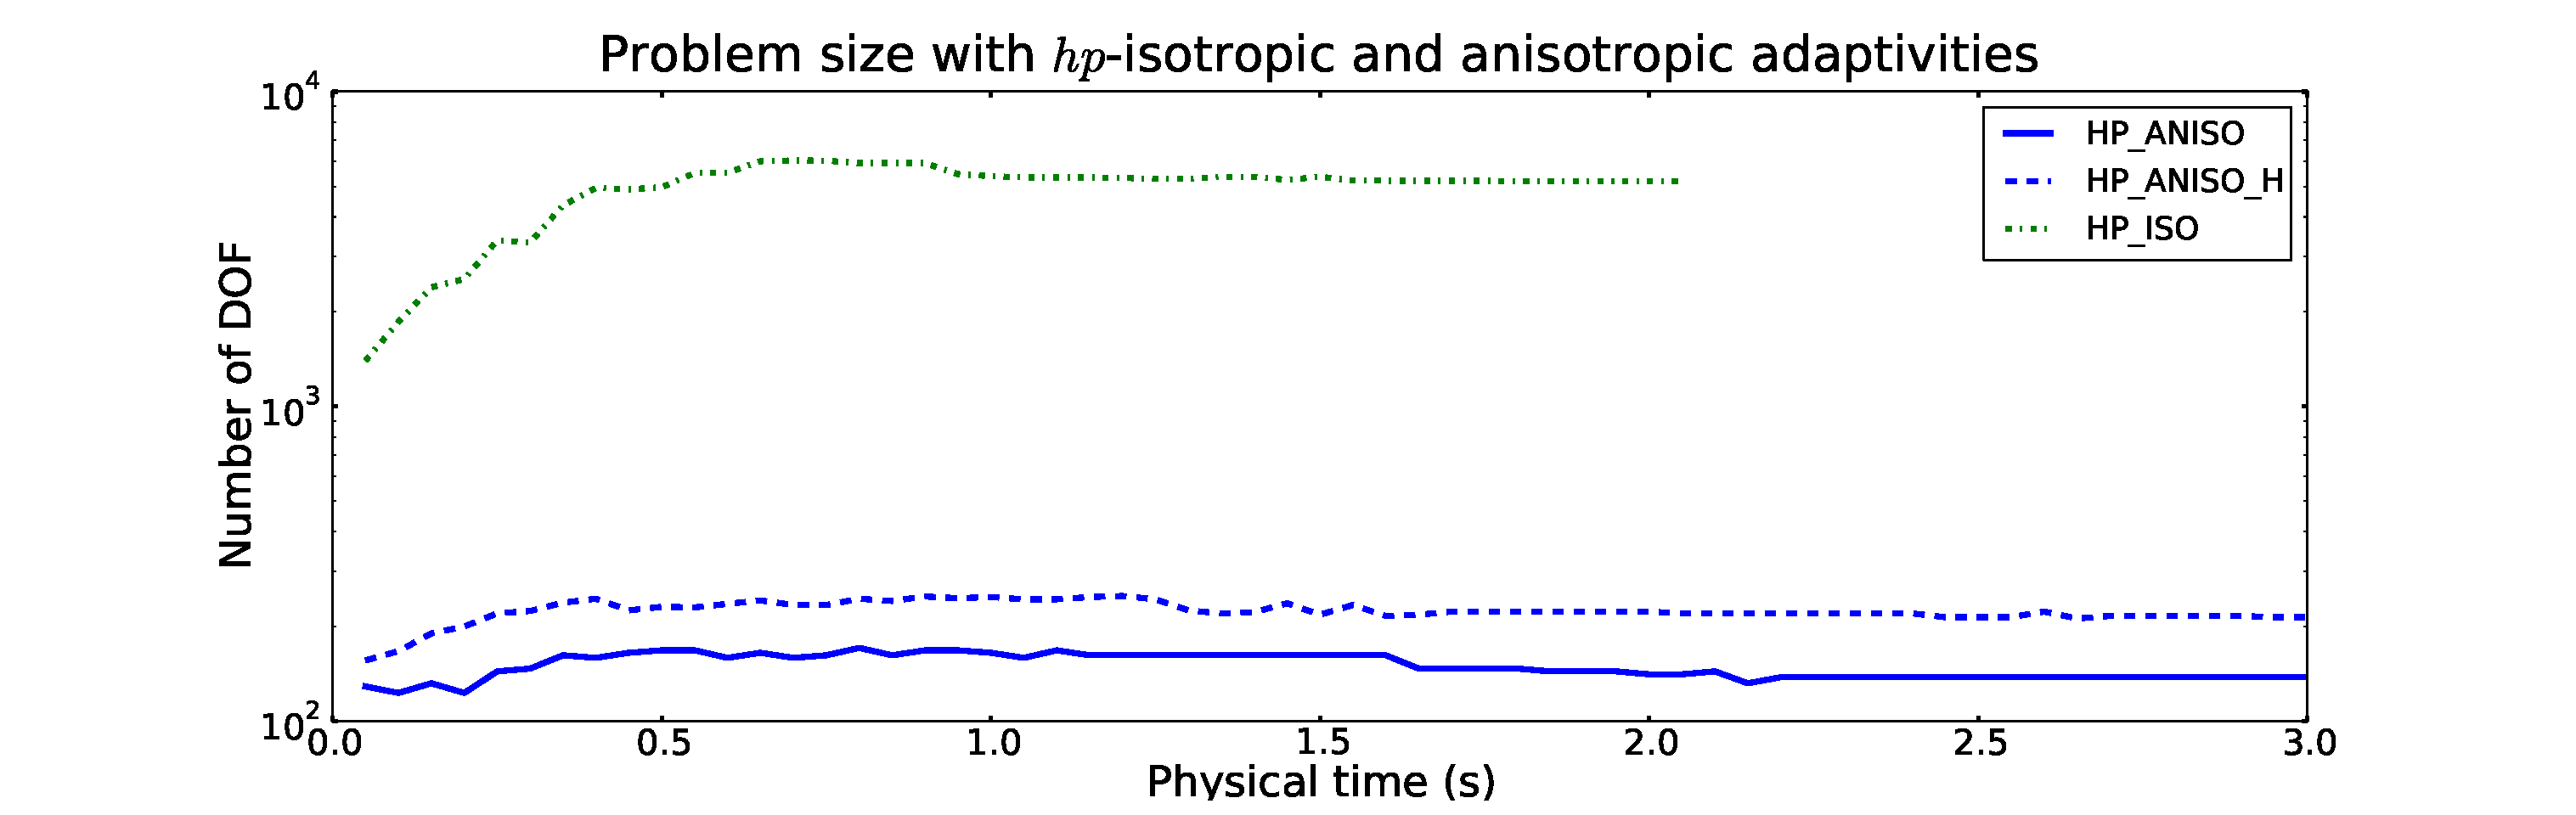
\includegraphics[width=\columnwidth]{isoaniso_dof}
  \caption{\label{fig:isoanisodof} NDOFs in case 
  of multi-mesh configuration with H\_ISO, H\_ANISO,
  HP\_ISO, HP\_ANISO, and single-mesh configuration with HP\_ANISO\_H
  refinement modes. (Notice log Y scale)}
  \end{centering}
\end{figure}

\begin{figure}[!ht]
  \begin{centering}
  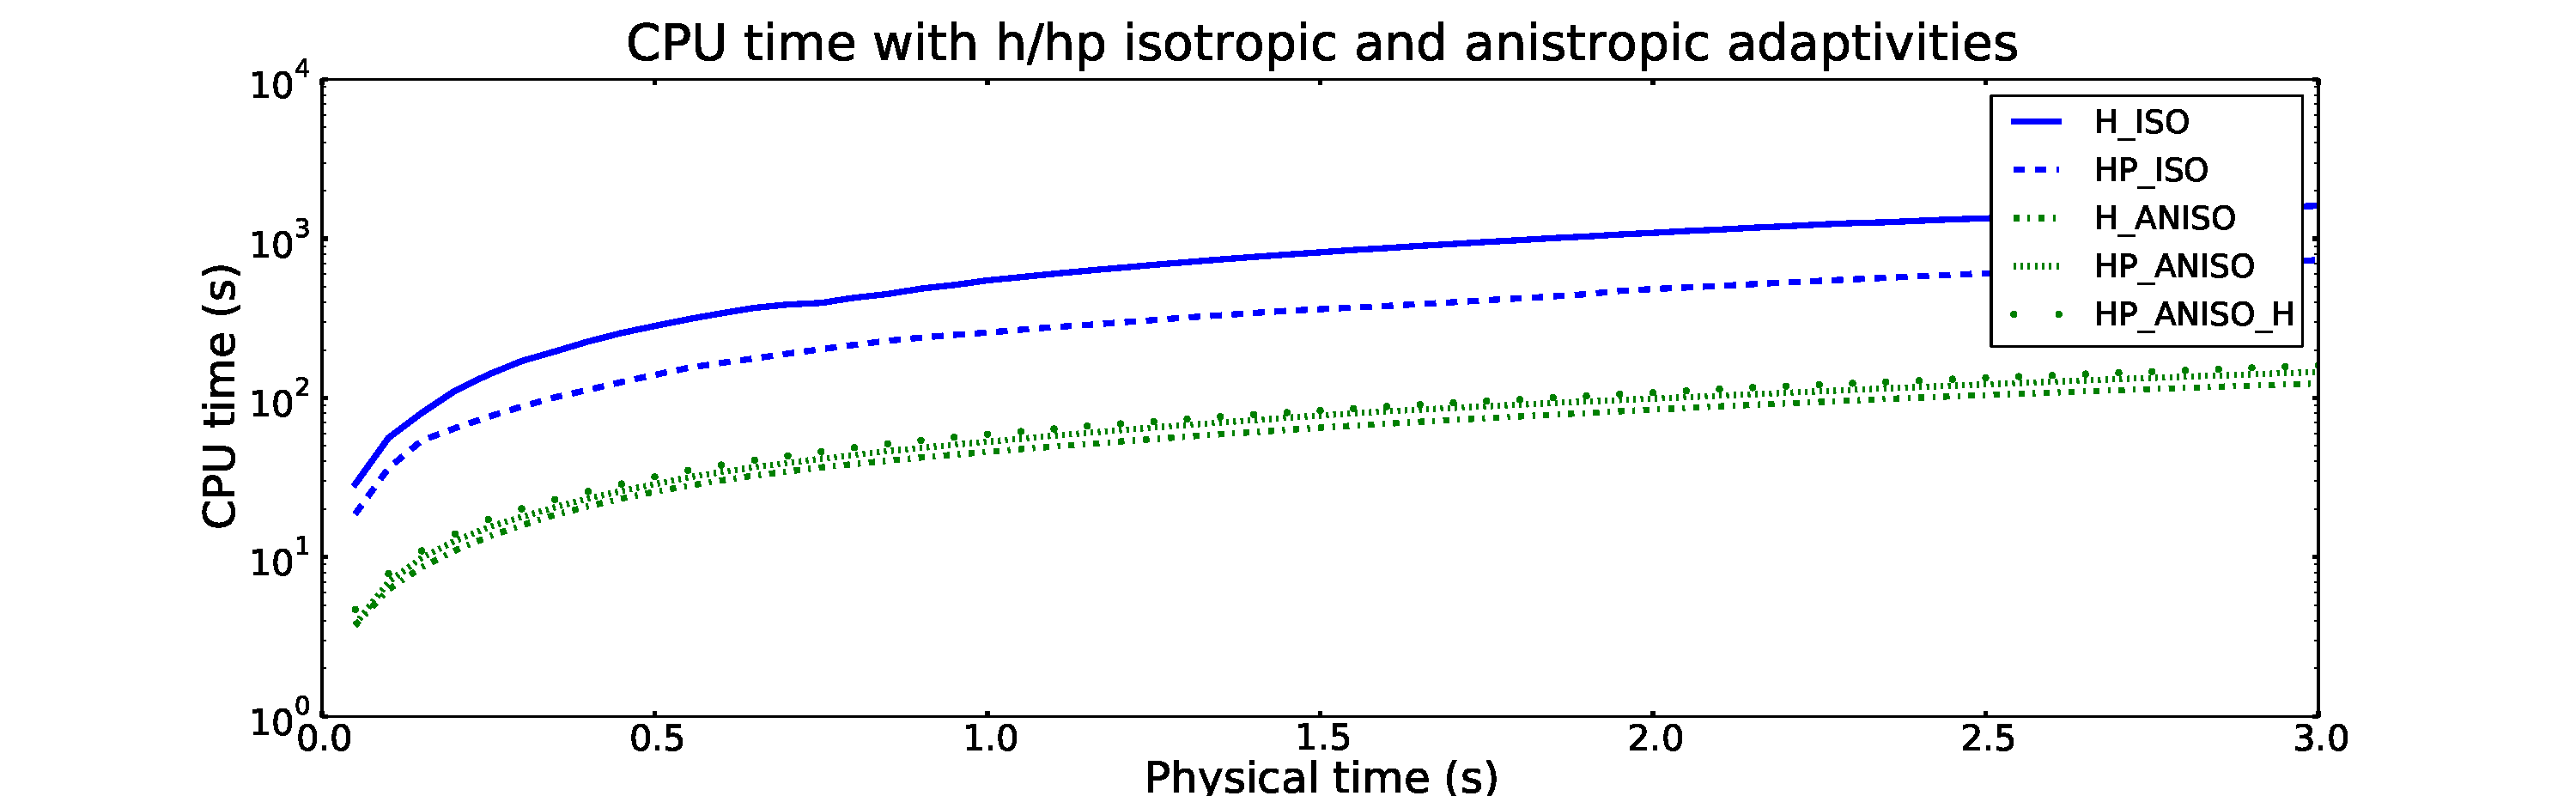
\includegraphics[width=\columnwidth]{isoaniso_cpu}
  \caption{\label{fig:isoanisocpu} Cumulative CPU times in case 
  of multi-mesh configuration with H\_ISO, H\_ANISO,
  HP\_ISO, HP\_ANISO, and single-mesh configuration with HP\_ANISO\_H
  refinement modes. (notice log Y scale)}
  \end{centering}
\end{figure}

\begin{figure}[!ht]
  \begin{centering}
  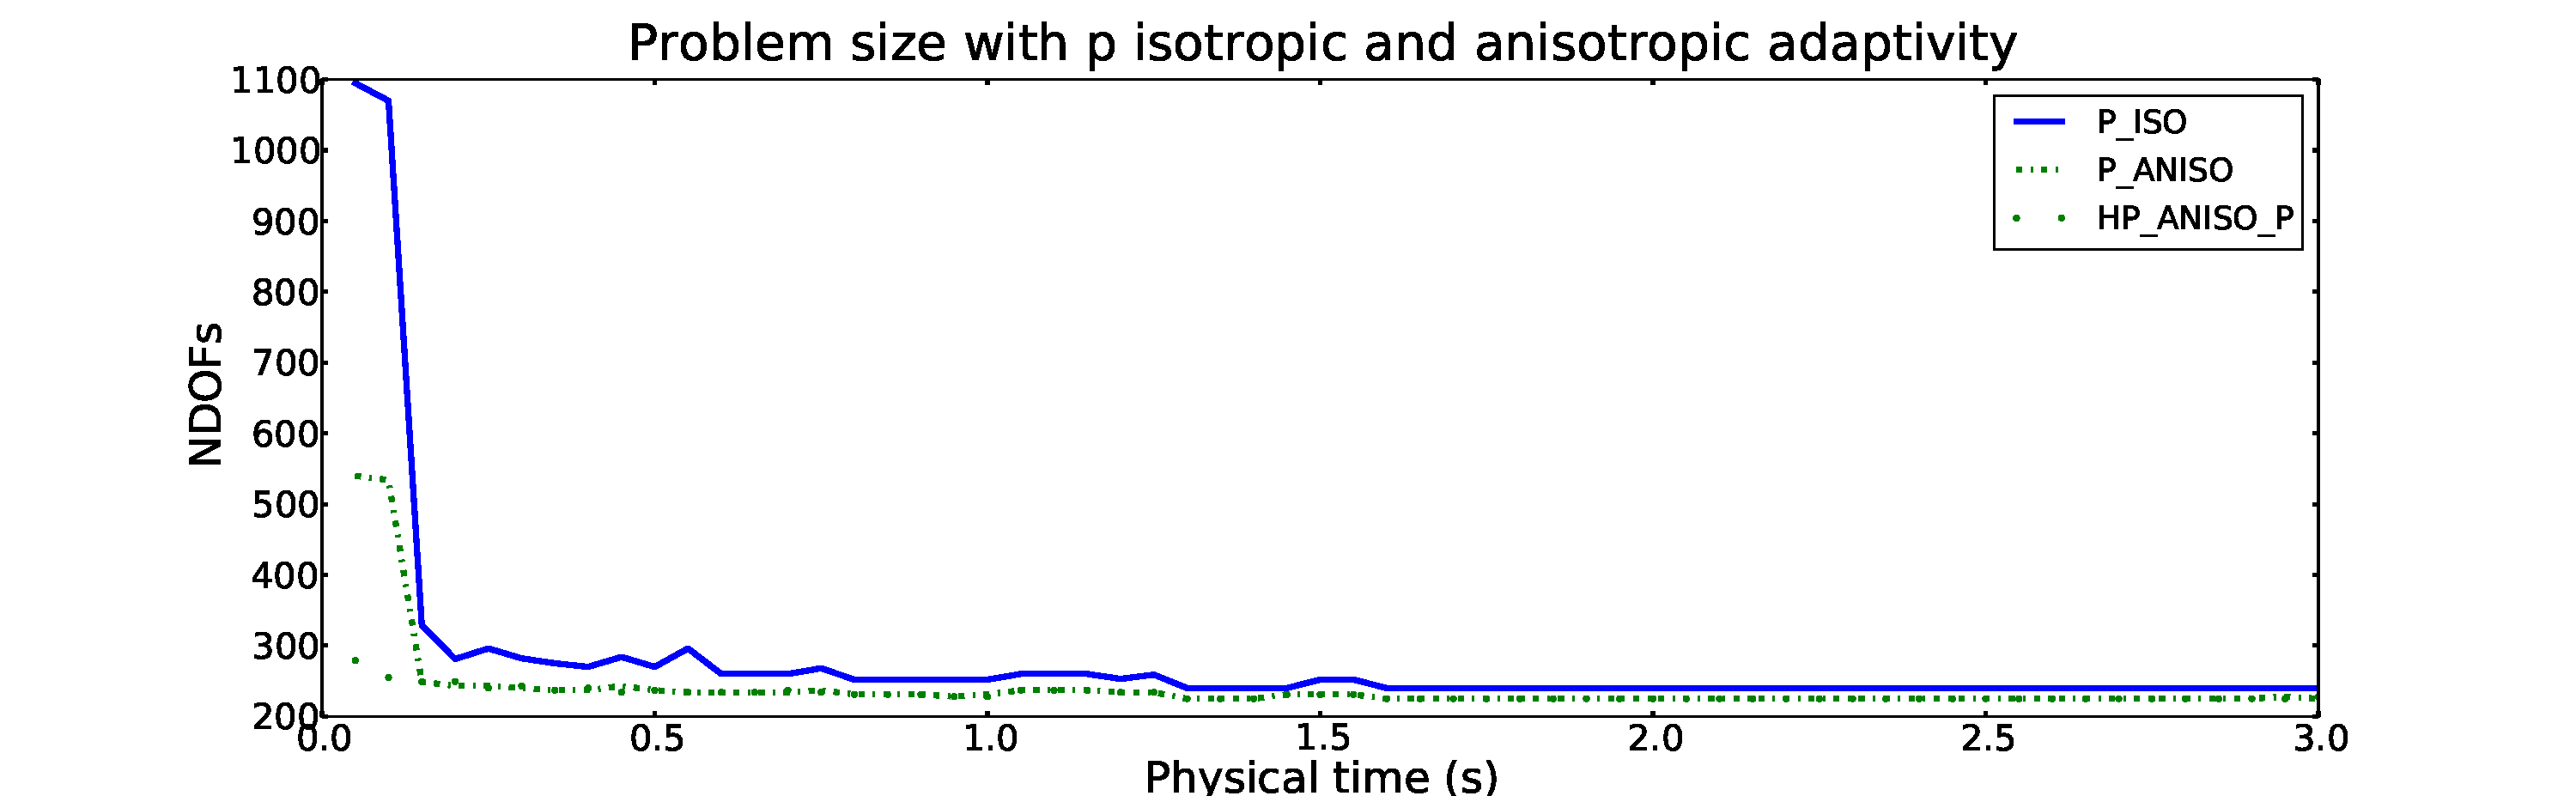
\includegraphics[width=\columnwidth]{isoanisop_dof}
  \caption{\label{fig:isoanisopdof} NDOFs in case 
  of multi-mesh configuration with P\_ISO, P\_ANISO, and
  HP\_ANISO\_P refinement modes.}
  \end{centering}
\end{figure}

\begin{figure}[!ht]
  \begin{centering}
  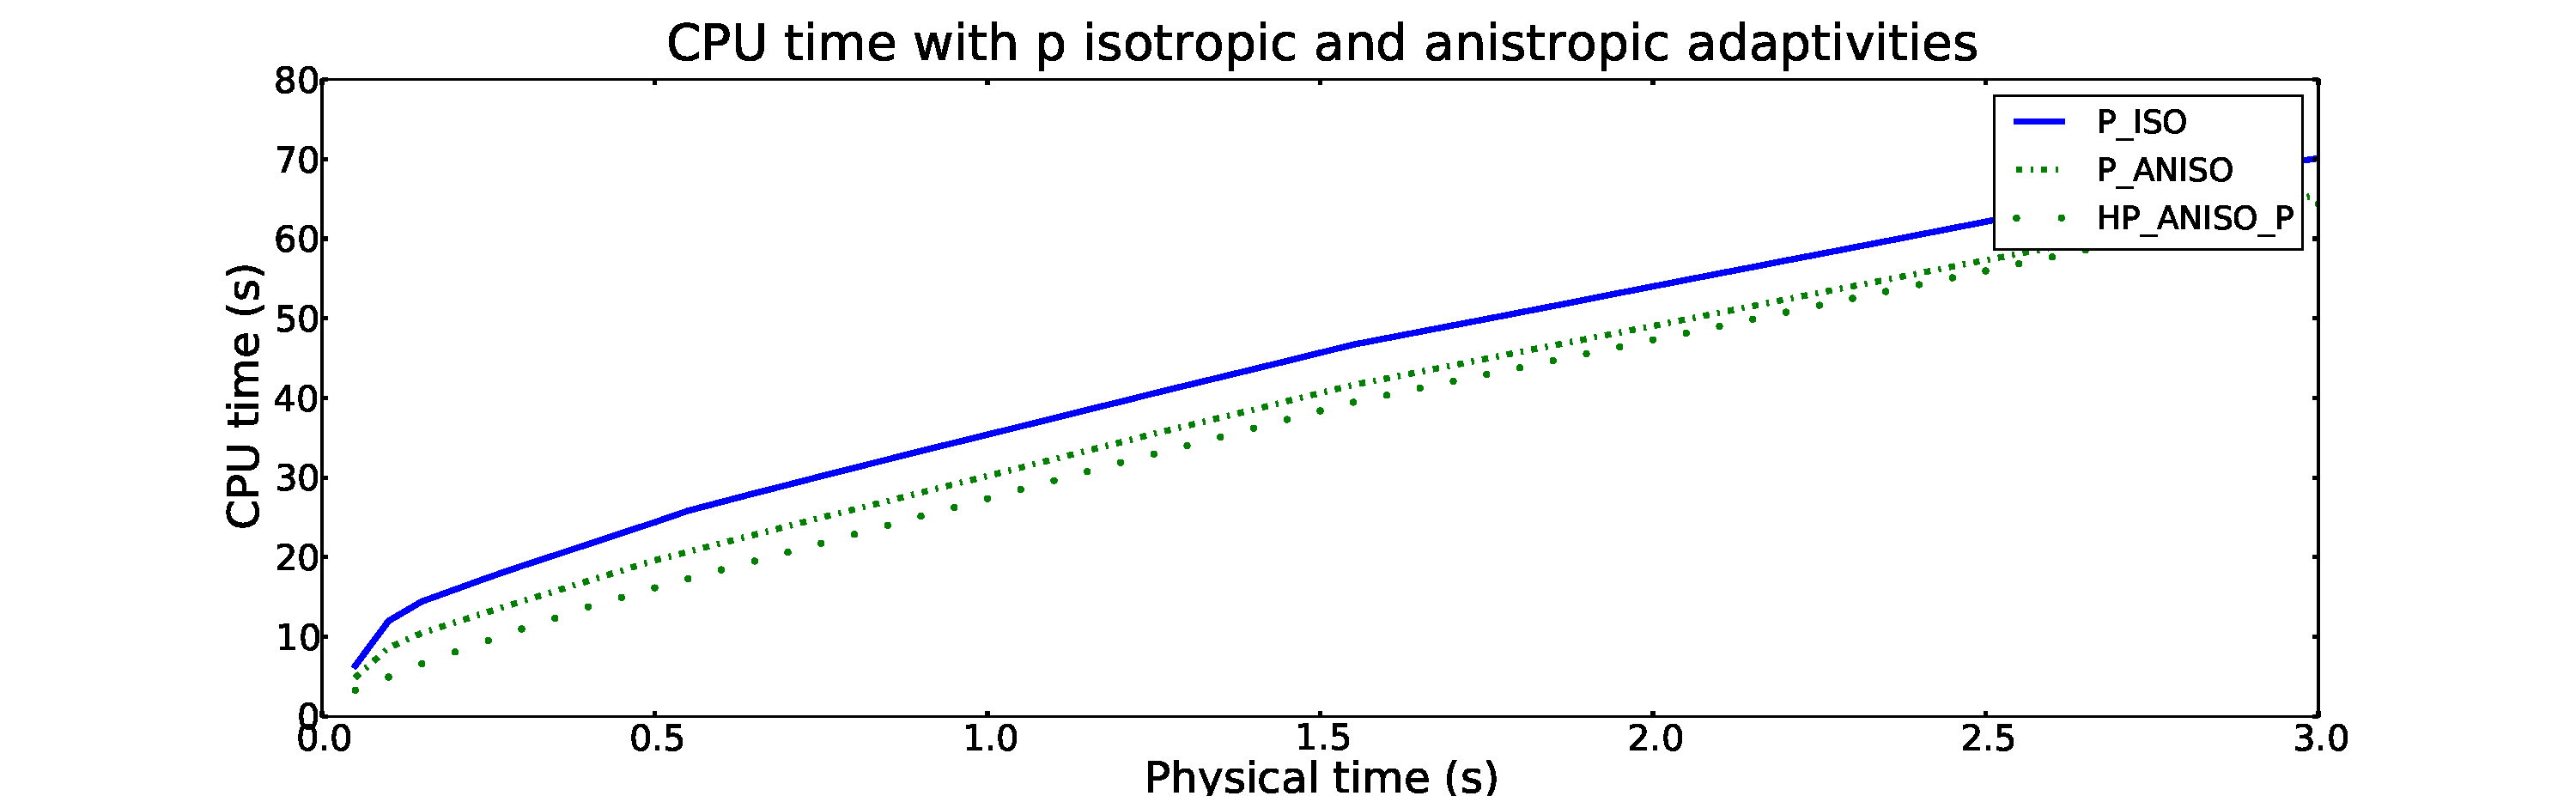
\includegraphics[width=\columnwidth]{isoanisop_cpu}
  \caption{\label{fig:isoanisopcpu} Cumulative CPU times in case 
  of multi-mesh configuration with P\_ISO, P\_ANISO, and
  HP\_ANISO\_P refinement modes.}
  \end{centering}
\end{figure}
To narrow down the list of refinement modes for the given problem, first the
isotropic and anisotropic adaptivities were compared. The \emph{p}-adaptivity
modes were compared separately as they used more refined initial mesh 
(shown in Fig.~\ref{fig:mesh}~(c)).
Fig.~\ref{fig:isoanisodof} and Fig.~\ref{fig:isoanisocpu} provide the comparison
of H\_ISO, H\_ANISO, HP\_ISO, HP\_ANISO, and HP\_ANISO\_H modes in terms of 
cumulative CPU time and NDOFs.
Fig.~\ref{fig:isoanisopdof} and Fig.~\ref{fig:isoanisopcpu} show the similar
comparsion for the P\_ISO, P\_ANISO, and HP\_ANISO\_P modes.
It is not difficult to see that the anisotropic refinement modes result in a reasonable problem
size and the problems solve within a reasonable calculation time. It is interesting
to note that HP\_ANISO results in the smallest problem size. Also, in
\emph{p}-adaptivity group, HP\_ANISO\_P results in the smallest problem size
at each time step, whereas P\_ISO and P\_ANISO result in a very large problem size
during the first time steps of the solution.
Here the term ``reasonable problem size''
means that the number of degrees of freedom in time converges
to so that $N_{DOF}<500$, and the term ``reasonable calculation time''
means that the calculation (step $\tau=0.01\ s$, physical
time $t_{end}=3.0\ s$) time $t$ on a givem system was $t<500\ s$.
Although these parameters are empirical, they serve as an upper limit, given
that the most refinement modes give significantly better results ---
$t<<500\ s$ and $N_{DOF} << 500$.

\subsection{Quantitative analysis of the refinement modes}

Based on the results in the previous subsection, H\_ANISO, HP\_ANISO,
and HP\_ANISO\_H from the \emph{hp/h}-adaptivity group and HP\_ANISO\_P
from \emph{p}-adaptivity group will be compared
in terms of NDOFs and cumulative CPU time. 
In all of the cases, the relative 
error at each time step remained below
the threshold which was set to $e_{th}=0.5\%$ between the coarse mesh
and fine mesh solutions, therefore the error-time plot will not be considered.

\begin{figure}[!ht]
  \begin{centering}
  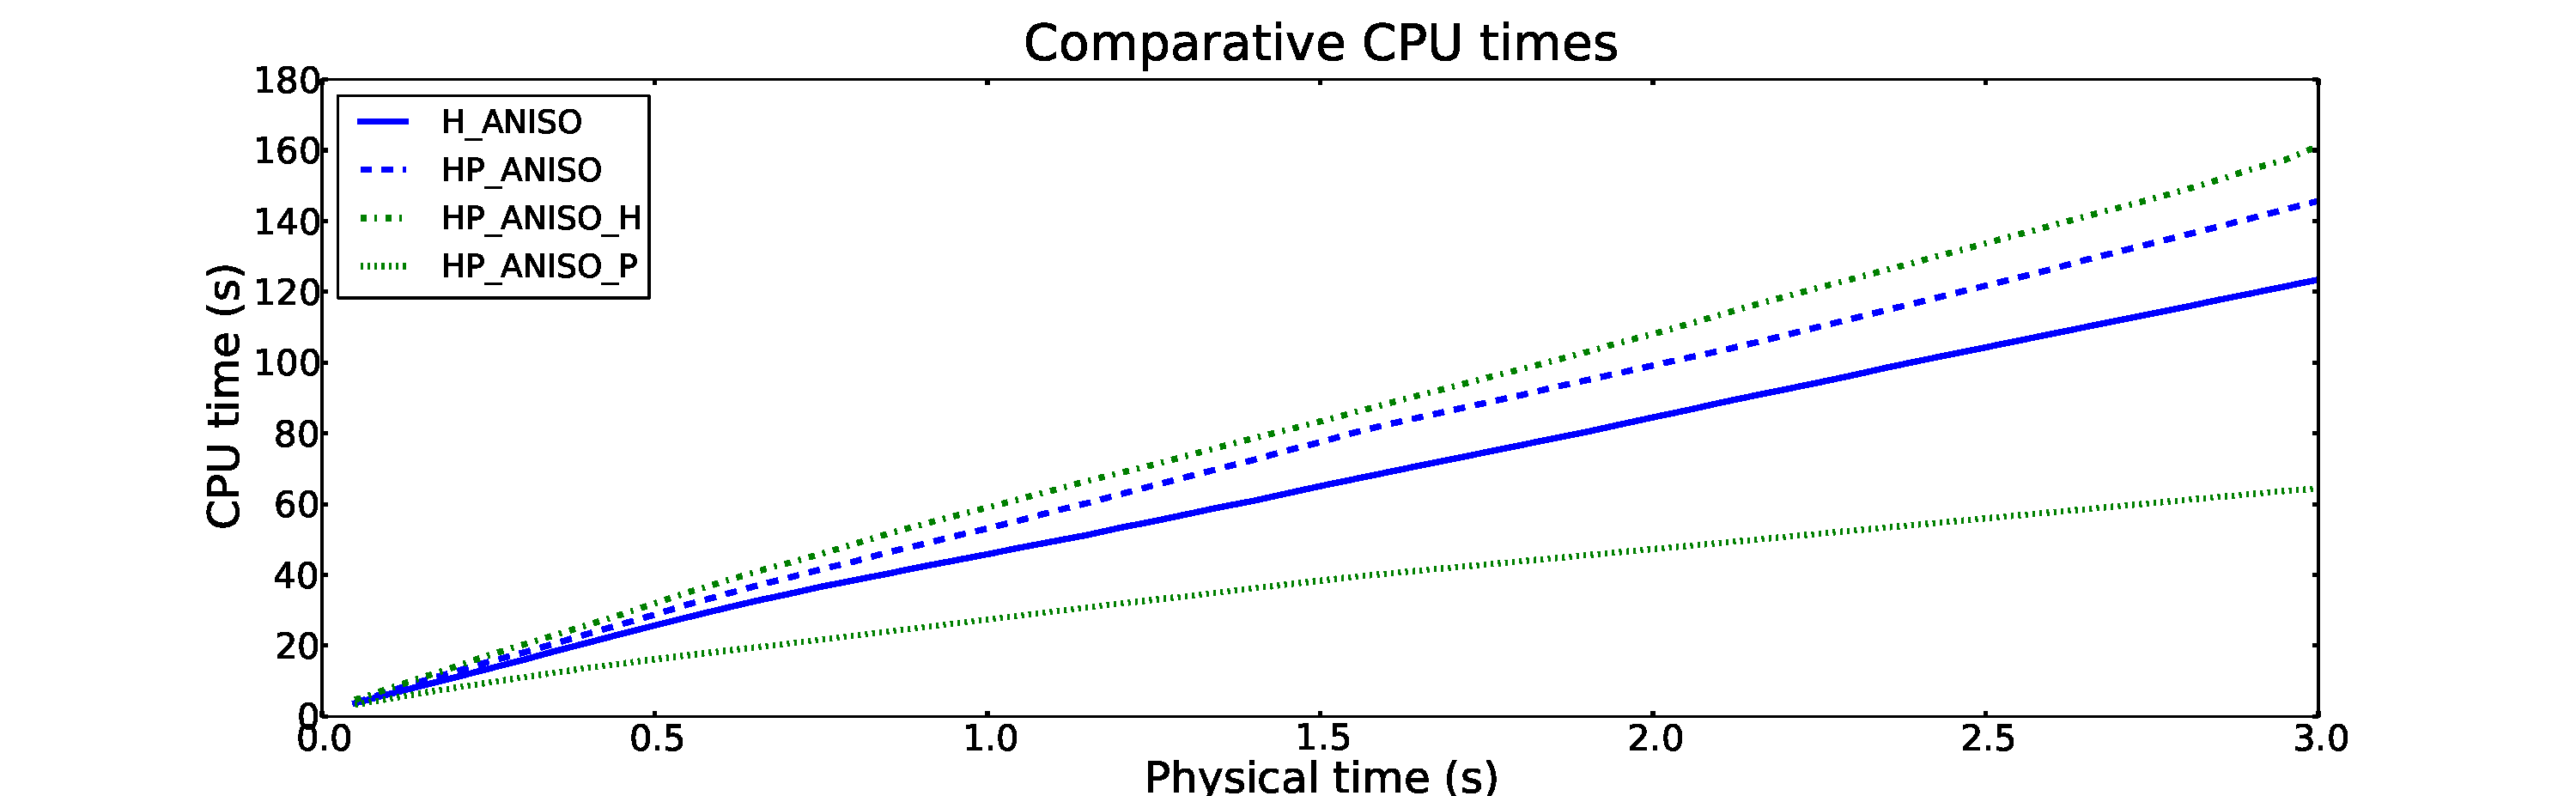
\includegraphics[width=\columnwidth]{cpu}
  \caption{\label{fig:cpu} Comparative cumulative CPU time for different refinement modes.}
  \end{centering}
\end{figure}

\begin{figure}[!ht]
  \begin{centering}
  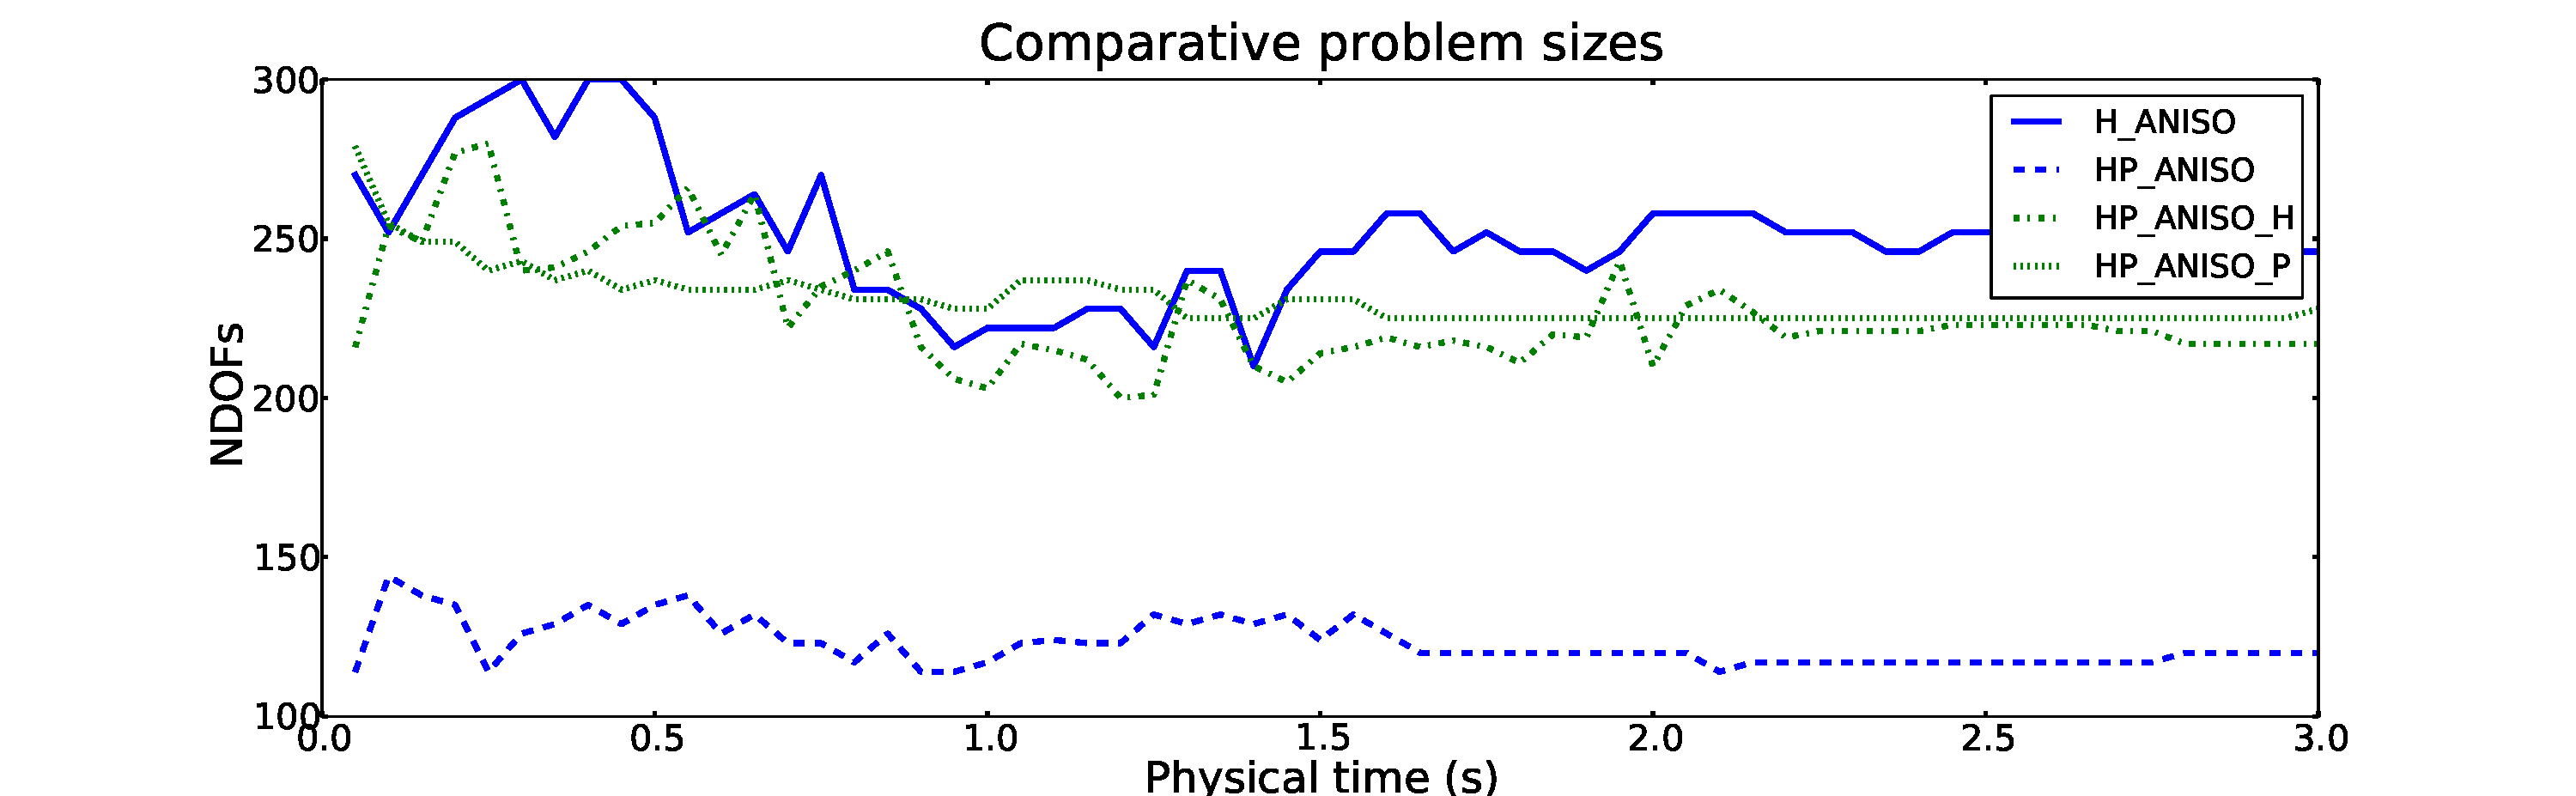
\includegraphics[width=\columnwidth]{dof}
  \caption{\label{fig:dof} Comparative NDOFs at each time step for 
  different refinement modes.}
  \end{centering}
\end{figure}

Fig.~\ref{fig:cpu} shows the cumulative CPU time for different refinement 
modes at each time step --- the results were recorded on the same computer
for the CPU times to be comparable.
We see that HP\_ANISO\_H and HP\_ANISO require the most
resources. This can be understood from the fact that in case of these 
refinement modes the adaptivity algorithm has the largest number of 
candidates (see Section.~\ref{sec:model} and Fig.~\ref{fig:refinements})
from which a particular refinement can be chosen.
At the same time, HP\_ANISO\_P is the fastest compared to the other refinement modes.
This can be attributed to the finer inital mesh.

Fig.~\ref{fig:dof} shows the NDOFs at each time step.
It can be seen that the HP\_ANISO results in the 
smallest problem size --- $N_{DOF} \approx 125$. 
All the other refinement modes result in a 
problem size of approximately ($N_{DOF} \approx 250$). Therefore
the HP\_ANISO is the most efficient in terms of memory consumption.

As we have filtered out
two notable refinement modes for the given problem --- HP\_ANISO\_P because of the fast
calculation, and HP\_ANISO because of the small problem size. In the following
subsection, some optimizations to reduce the CPU time of
HP\_ANISO and reduce the NDOFs of HP\_ANISO\_P will be considered.


\subsection{Optimizations of HP\_ANISO and HP\_ANISO\_P refinement modes}

\begin{figure}[!ht]
  \begin{centering}
  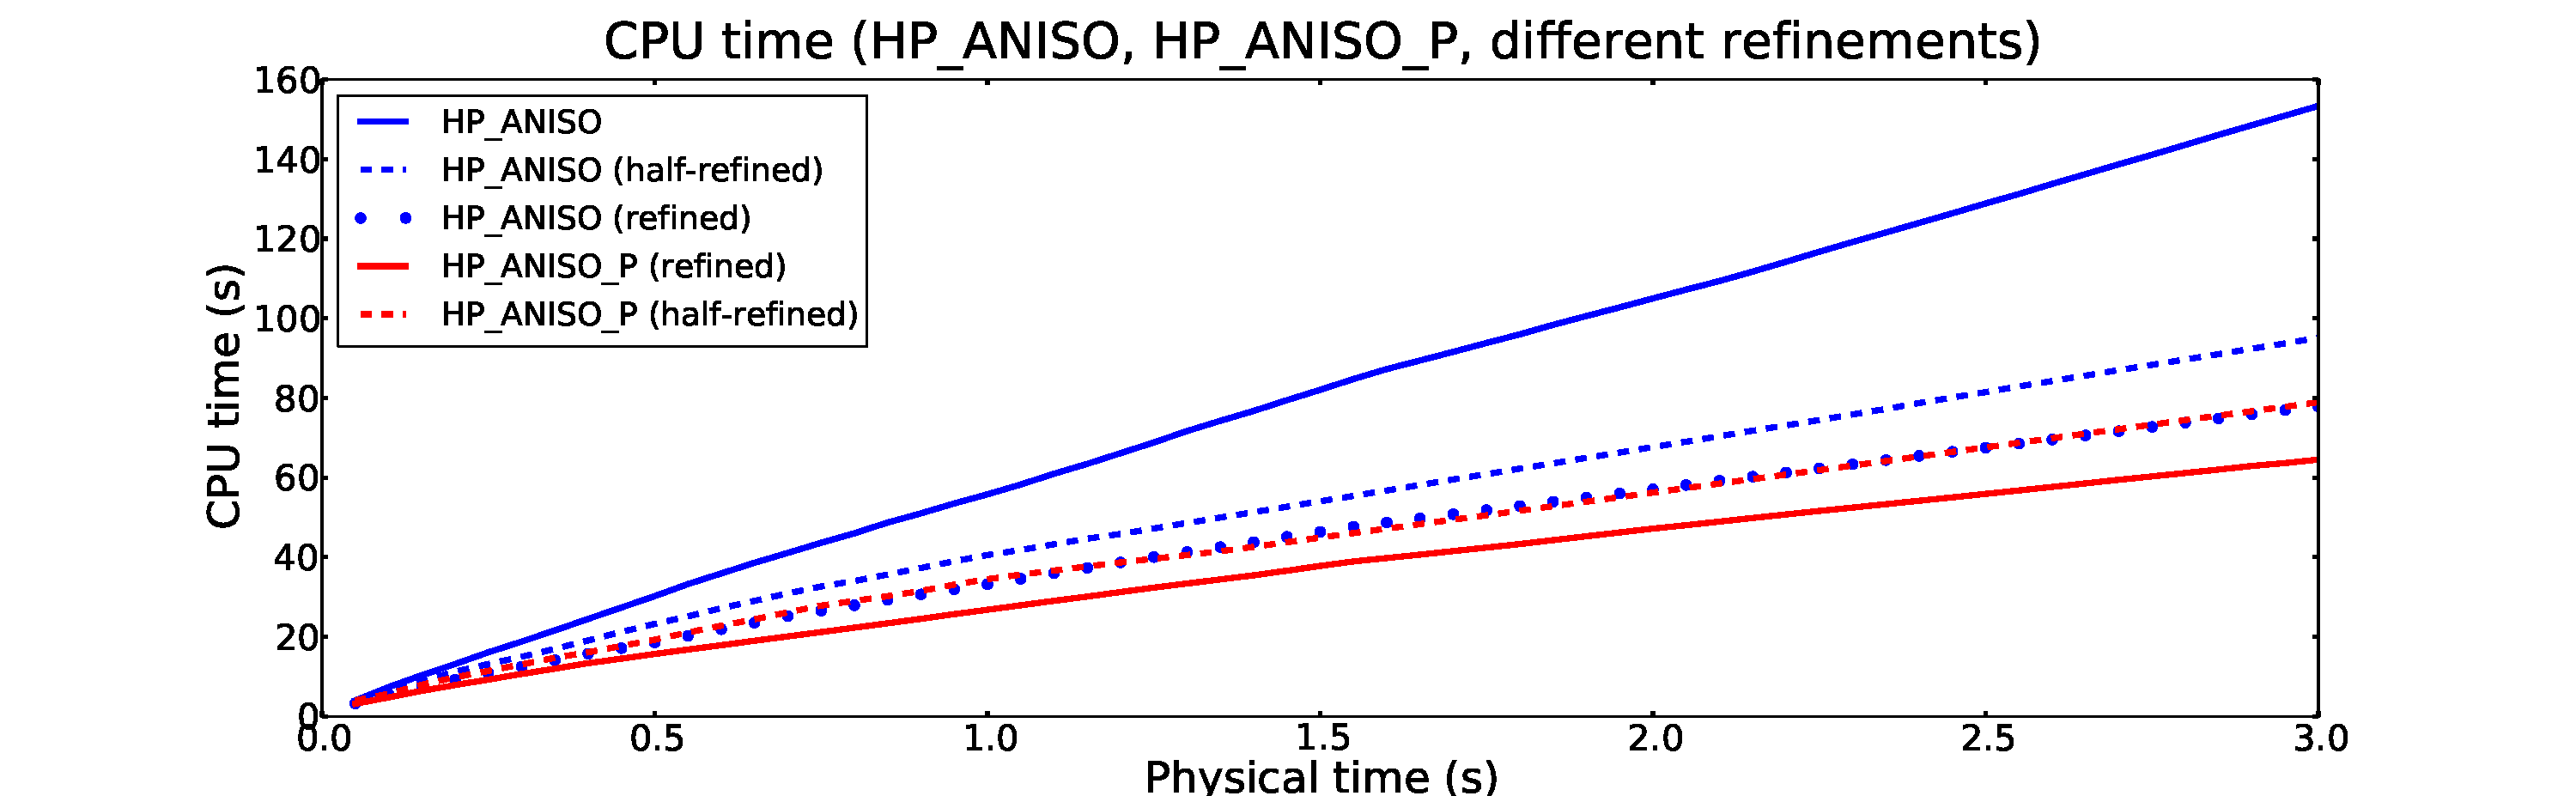
\includegraphics[width=\columnwidth]{refined_cpu}
  \caption{\label{fig:refined-cpu} Cumulative CPU time for HP\_ANISO and HP\_ANISO\_P
  with different initial meshes.}
  \end{centering}
\end{figure}

\begin{figure}[!ht]
  \begin{centering}
  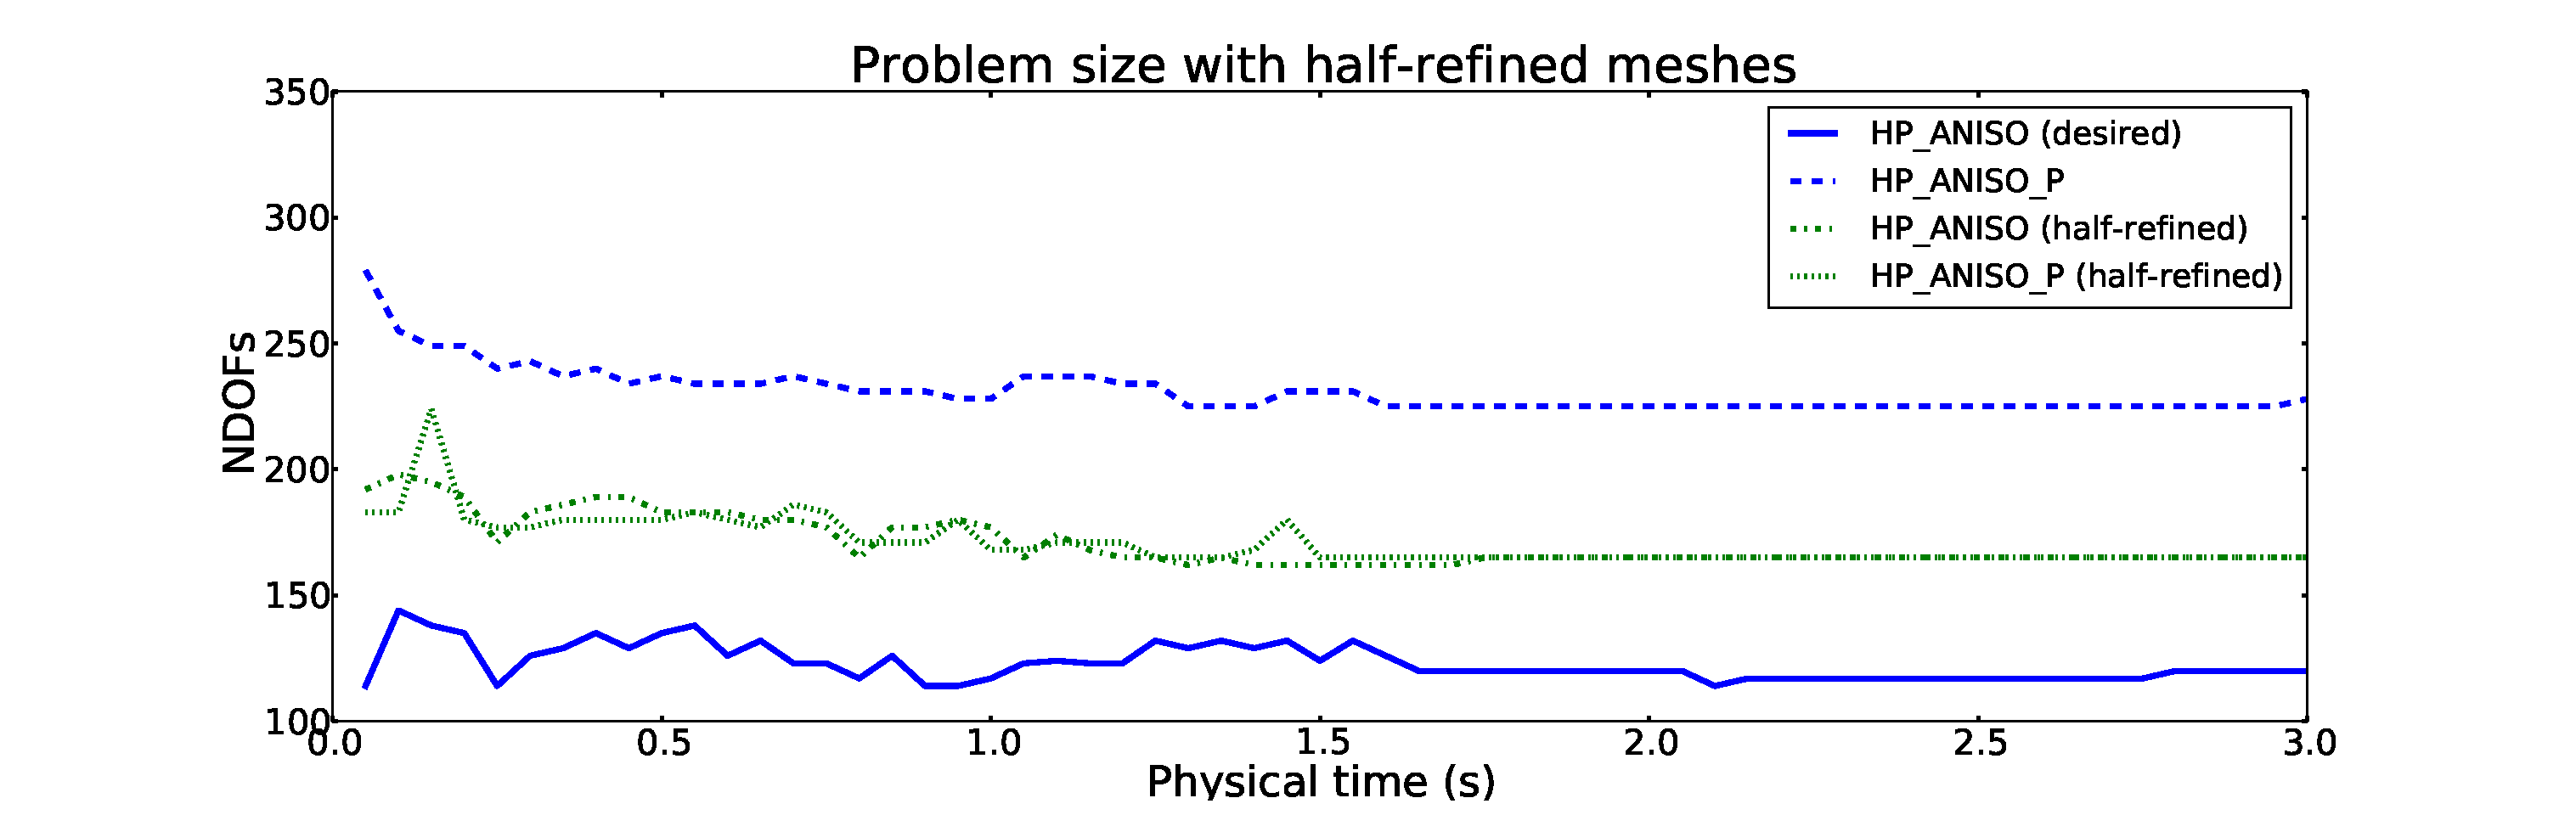
\includegraphics[width=\columnwidth]{refined_dof}
  \caption{\label{fig:refined-dof} NDOFs at each time step for
  HP\_ANISO and HP\_ANISO\_P with different meshes.}
  \end{centering}
\end{figure}

When it comes to a large domain or 3D modeling, the problem
size becomes a very important factor. Namely, 3D full scale solutions tend to use
a lot of memory. Therefore, we consider HP\_ANISO the most
suitable refinement mode for the given problem. 
Hence, some ways to optimize the HP\_ANISO model
to improve the CPU time factor without significantly 
compromising the NDOFs will be considered. 
The desirable output would be HP\_ANISO problem size
close to HP\_ANISO\_P CPU time. 
One way to optimize the problem
is to choose more refined initial mesh. Another way would be to change
the refinement frequency during the solving process. Theoretically it 
could result in a fewer adaptivity steps which are rather expensive in terms
of CPU time. Recall that up to this point,
the initial mesh was loaded in the beginning of each time step. 
True, by employing the optimizations, one must know something about the problem
and its solution beforehand. However, it could still be practial when solving a real problem
in a large domain.

The problem size and CPU time with HP\_ANISO
and HP\_ANISO\_P adaptivities on more refined initial mesh (see Fig.~\ref{fig:mesh}~(c))
compared to the coarse initial mesh (Fig.~\ref{fig:mesh}~(a)) and 
HP\_ANISO\_P solution are shown in Fig.~\ref{fig:refined-cpu} and Fig.~\ref{fig:refined-dof}.
By using initially more refined mesh, the problem solving time
can be reduced in case of HP\_ANISO, at the same time, the problem size increases
as the initial mesh is not necessarily the most optimal one.
However, in this situation, HP\_ANISO\_P and HP\_ANISO perform equally well.

\begin{figure}[!ht]
  \begin{centering}
  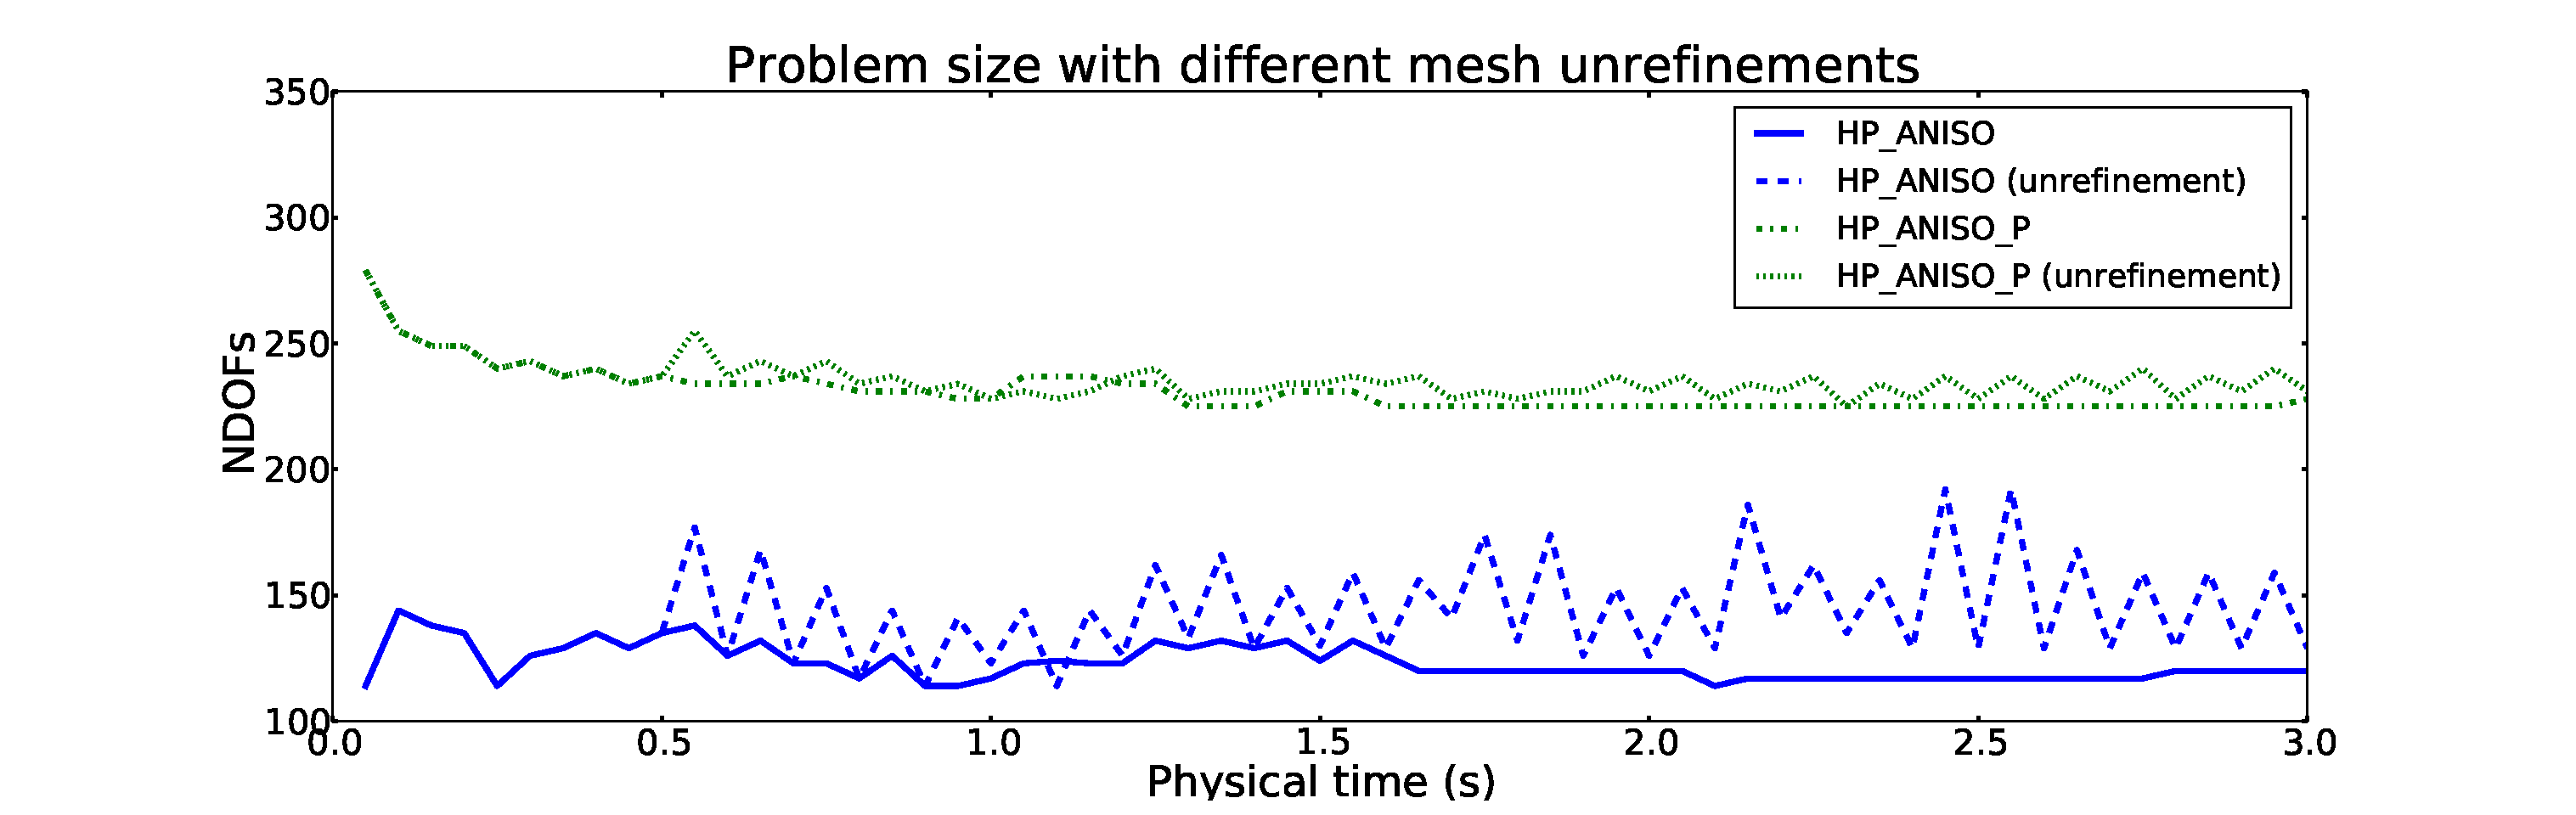
\includegraphics[width=\columnwidth]{unreffreq_dof}
  \caption{\label{fig:unreffreq-dof} NDOFs at each time step for
  HP\_ANISO and HP\_ANISO\_P with mesh unrefinement at each time step and at over each
  	time step after first $0.5\ s$ physical solution time.}
  \end{centering}
\end{figure}
The next proposed optimization involved changing the unrefinement frequency.
It is known that the concentration gradient $\nabla C$ changes the most in the initial phase
of the calculation, therefore, the unrefinement after each time step was performed
until $t=0.5\ s$ (physical time). After that, the
unrefinement was performed in $\Delta t = 0.10\ s$ interval.
However, this optimization does not appear to result in a stable solution, 
i.e. the problem size 
does not remain steady, but starts to oscillate depending on the unrefinement
frequency. This is shown in Fig.~\ref{fig:unreffreq-dof}. 

Therefore varying the unrefinement frequency will
likely not result in desired results in real applications for given system of equation.
At the same time, by varying the initial mesh size, optimal initial mesh could be found
for both HP\_ANISO and HP\_ANISO\_P refinement modes.
	 
\subsection{More general results}
\begin{figure}[!ht]
  \begin{centering}
  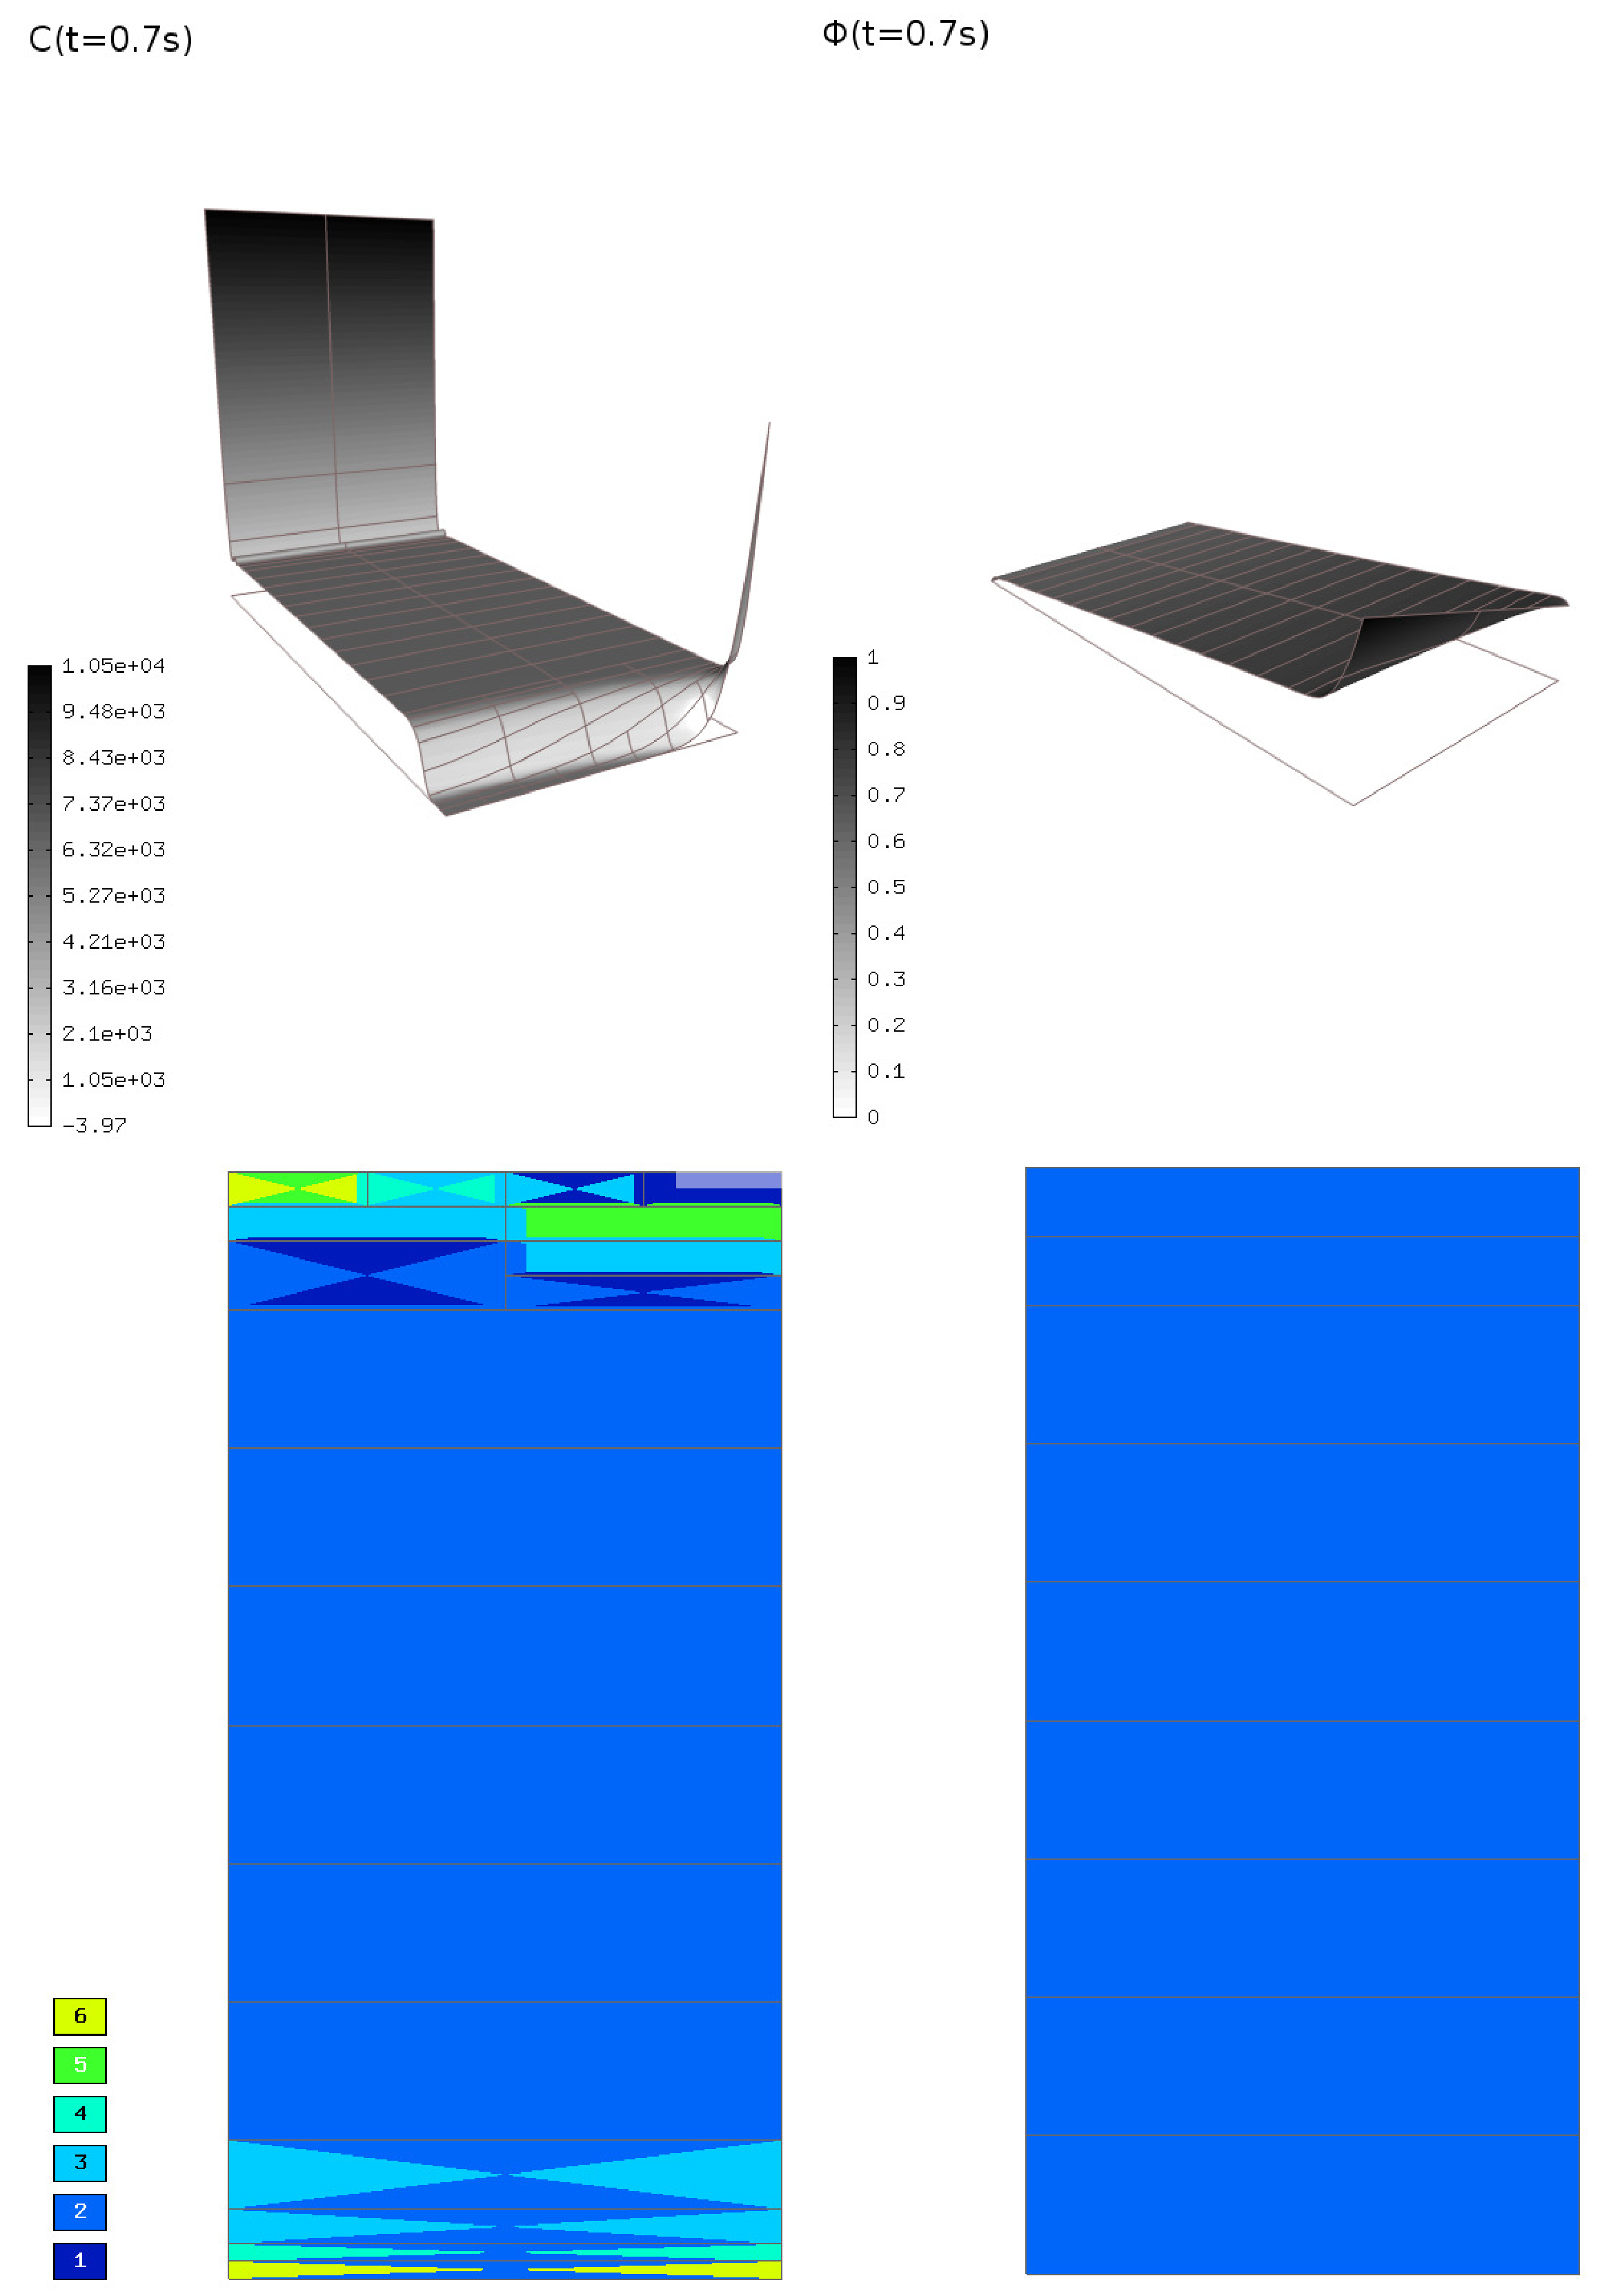
\includegraphics[width=.75\columnwidth]{cphiorders}
  \caption{\label{fig:cphi-orders} Solutions $C$ and $\phi$
  and corresponding polynomial degrees of the elements at
  $t=0.7\ s$. HP\_ANISO refinement mode was used. The height
  in the solution graphs indicates the value.}
  \end{centering}
\end{figure}

Based on the results, cation concentration and voltage was calculated
for different boundary conditions.
For instance, when voltage is applied as follows
\begin{equation}
  \phi_{\Omega_1}=0.5\frac{x}{width_{\Omega_1}}+0.5,
\end{equation}
the concentration gradient $\nabla C$ and the voltage gradient $\nabla \phi$ are no
longer effectively 1D.
The calculated $C$ and $\phi$ in $\Omega$ and corresponding meshes and polynomial
degrees of the elements are shown in Fig.~\ref{fig:cphi-orders}.
HP\_ANISO refinement mode was used. Notice that the solution
is different to the one in Fig.~\ref{fig:cphi} and the adapted mesh and the
polynomial degrees are also more complicated than in Fig.~\ref{fig:poly}.
It must be noted that in case of non uniform boundary conditions which
results in 2D problem, refined initial mesh was more efficient to use.
